\section{Momentum Reconstruction}\label{subsec:MomRecon}

The algorithm to reconstruct particle momentum in CC-$1\pi$ analysis
integrates the average energy deposition per unit of areal density
along the track through the \podtext{}. The path of the track is determined
by the energy depositions in each scintillator plane of the \podtext{}
associated with the reconstructed track object. The integration for
contained tracks is done starting at the end of the reconstructed
track, where the momentum is assumed to be close to zero to the start
position of the reconstructed track. In cases where the track exits
the \podtext{} into TPC1, the momentum calculated by TPC1 is used as the
starting momentum and the integration begins at the point where the
track exited the \podtext{}. (For this discussion the downstream ECal is
considered to be part of the \podtext{}, and the difference in areal density
is taken into consideration.) Events with tracks that exit the \podtext{}
but do not enter TPC1 (do not have a matched track in TPC1) are
excluded from the analysis.


Relativistic particles will generally deposit energy as Minimum
Ionizing Particles (MIPs) as characterized by the Bethe-Bloch curve in~(\ref{eqn:bethebloch})

\begin{align}\label{eqn:bethebloch}
    -\frac{dT}{dx} &= K z^2\frac{Z}{A} \frac{1}{\beta^2}\left[\frac{1}{2}\ln\left(\frac{2 m_{e}c^{2}{(\beta\gamma)}^{2}T_\text{max}}{I^2}\right) - \beta^{2} - \frac{\delta\left(\beta\gamma\right)}{2}\right] \\
    \text{~with} \nonumber \\
    T_\text{max} &= \frac{2 m_{e}c^{2}{(\beta\gamma)}^{2}}{1+2\gamma \frac{m_e}{M} + {\left(\frac{m_e}{M}\right)}^2} \nonumber
\end{align}

\noindent{}where $T$ is the kinetic energy, $x$ is the distance
traveled, $K$ is proportional to the material density, $I$ is the mean
excitation potential in eV, $z$ is the charge, $c$ is the speed of
light, $M$ is the rest mass of the particle, $m_{e}$ is the rest mass
of the electron, $\beta$ is the velocity as a fraction of $c$, and
$\gamma$ is the Lorentz relativistic factor
${\left(1-\beta^{2}\right)}^{-0.5}$.  Both muons ($m_{\mu} =
105.6\text{~MeV}/c^{2}$) and pions ($m_{\pi} = 139.5
\text{~MeV}/c^{2}$) are relativistic at the energies required to be
detected and reconstructed by the \podtext{}.

\subsection{Momentum Tool}

The Momentum Tool (MT), the collection of functions that estimate a
particle's momentum in the \podtext{}, was initially developed to estimate
the kinetic energy of protons fully contained in the \podtext{}. The MT
estimated the proton's momentum by summing up the assumed ionization
energy loss in each material traversed over the range of the track in
the \podtext{}. Stopping power data for different materials
came from the NIST PSTAR catalog as a function of kinetic
energy. The MT was extended to
measurements of muon and pion momenta for tracks originating in the
\podtext{} and entering TPC1.  The extension involved converting kinetic
energy to $\beta\gamma$ = $p/(Mc)$, the dimensionless quantity of a
particle's momentum divided by its mass.

The starting kinetic energy for the MT is given by (\ref{eqn:initialKinE}),

\begin{equation}\label{eqn:initialKinE}
    T_{i,\alpha} =
        \begin{cases}
            \sqrt{{(p_\text{TPC1}c)}^2 + {(m_\alpha c^2)}^2} - m_\alpha c^2 &\mbox{if }p_\text{TPC1} \neq 0 \,\\
            \epsilon_\alpha &\mbox{otherwise} \,
        \end{cases}
\end{equation}

\noindent{}where the index $\alpha$ denotes either a muon, proton, or
pion. The starting kinetic energy $\epsilon$ for muons and pions is 30
MeV and for protons is 50 MeV. A study showed that the resulting momentum
distributions for the muon and pion did not change when using a starting point smaller than
30 MeV.


The MT steps through the \podtext{} along the path defined by a collection of track-nodes.
A track-node is a collection of time-correlated hits inside active material
with charged-weighted position and direction. The direction vector points to
the next node except in the case of the last track-node, in which case, it uses
the previous node's direction. The positions of two successive nodes and
the associated direction vector determine the angle, $\theta$, of the
track w.r.t.~the \podtext{} z-axis. The MT numerically integrates the energy
loss for each material traversed in the following manner,

\begin{align*}
    \Delta~T &= {\left(\frac{dT}{d\rho_{A}}\right)}_\text{mat} {\left(\Delta\rho_{A}\right)}\\
    T &\rightarrow T+\Delta T \,
\end{align*}

\noindent{}where the index ``mat'' represents each material in the path,
$\rho_{A}$ is the areal density, and $\Delta\rho_{A}$ is a
small step of 0.05 gram/cm$^2$ in areal density. Each $\Delta\rho_{A}$ step in $dT/d\rho_{A}$ is
evaluated at the point $\beta\gamma$ $= {(\beta\gamma)}_0 +
\Delta(\beta\gamma)/2$ where ${(\beta\gamma)}_0$ is the value of $\beta\gamma$
for a single particle of kinetic energy $T$ and $\Delta(\beta\gamma)$ is the density correction term from~(\ref{eqn:bethebloch}).

\subsection{Momentum Calibration}\label{subsec:MomToolSubsamples}

The muon and pion track momenta were calibrated for all the track topologies in the analysis.
To avoid biasing the calibration to the NEUT generator kinematics,
the muon and pion tracks were selected from true events passing the particle idenfitication cuts.
Additionally, calibration training samples were extracted using subsets of the monte carlo (MC). Specifically,
about $1.16\times10^{21}$ POT from both water-in and water-out MC were used.
This is about $5\times$ and $3\times$ the data statistics for water-in and water-out modes, respectively, in the measurement.

A bias subtraction method is applied on each track to calibrate to the true
momentum. To characterize the momentum bias, a two-dimensional
histogram of the true-vs-reconstructed momenta over the full
particle's phase-space is created and used to generate a profile
histogram of the momentum bias as a function of the reconstructed
momentum. This profile histogram is also constructed with each bin to
have approximately equal statistics so as to minimize the impact of
statistical fluctuations. The profile is then carefully examined for
features, such as tails, maxima, or minima, in order to characterize
the shape with a function. Next a closed form function that reasonably describes
the shape of the bias is identified. The metric for a determining if
the chosen function is ``adequate'' is to require at least four bins in
the profile and that a chi-squared fit value is similar to the number of degrees of freedom.
Once the suitable functional form, $R$, is fitted to the profile
histogram, the calibrated momentum, $p_c$ is calculating using~(\ref{eqn:momentumcalibration})

\begin{equation}\label{eqn:momentumcalibration}
    p_c = [1 - R(p_r)] \times p_r\,
\end{equation}

\noindent{}where $p_r$ is the uncalibrated, raw momentum.

To illustrate the method of calibration, the calibration method for true CC-$1\pi$ muon tracks fully contained in the \podtext{}
is shown in Figure~\ref{fig:MuonContainedCalibration}.
There is better agreement between the true and reconstructed momenta, but additional variance is introduced.
The increase in the variance is expected since a bias corrections will introduce a larger spread to the momentum
distribution. The calibration function for this set is given by

\begin{equation*}
    R(p_{r}\text{\ [GeV/c]}) =  0.02955 + \frac{0.045662}{1+\exp\left[-24.61\left(p_r-0.4415\right)\right]}\,
\end{equation*}

\noindent{}and is shown in Figure~\ref{fig:MuonContainedResolutionProfile}.

\begin{figure}
    \begin{centering}
        \subfloat[True vs.\ uncalibrated momentum]
        {%
            \begin{centering}
                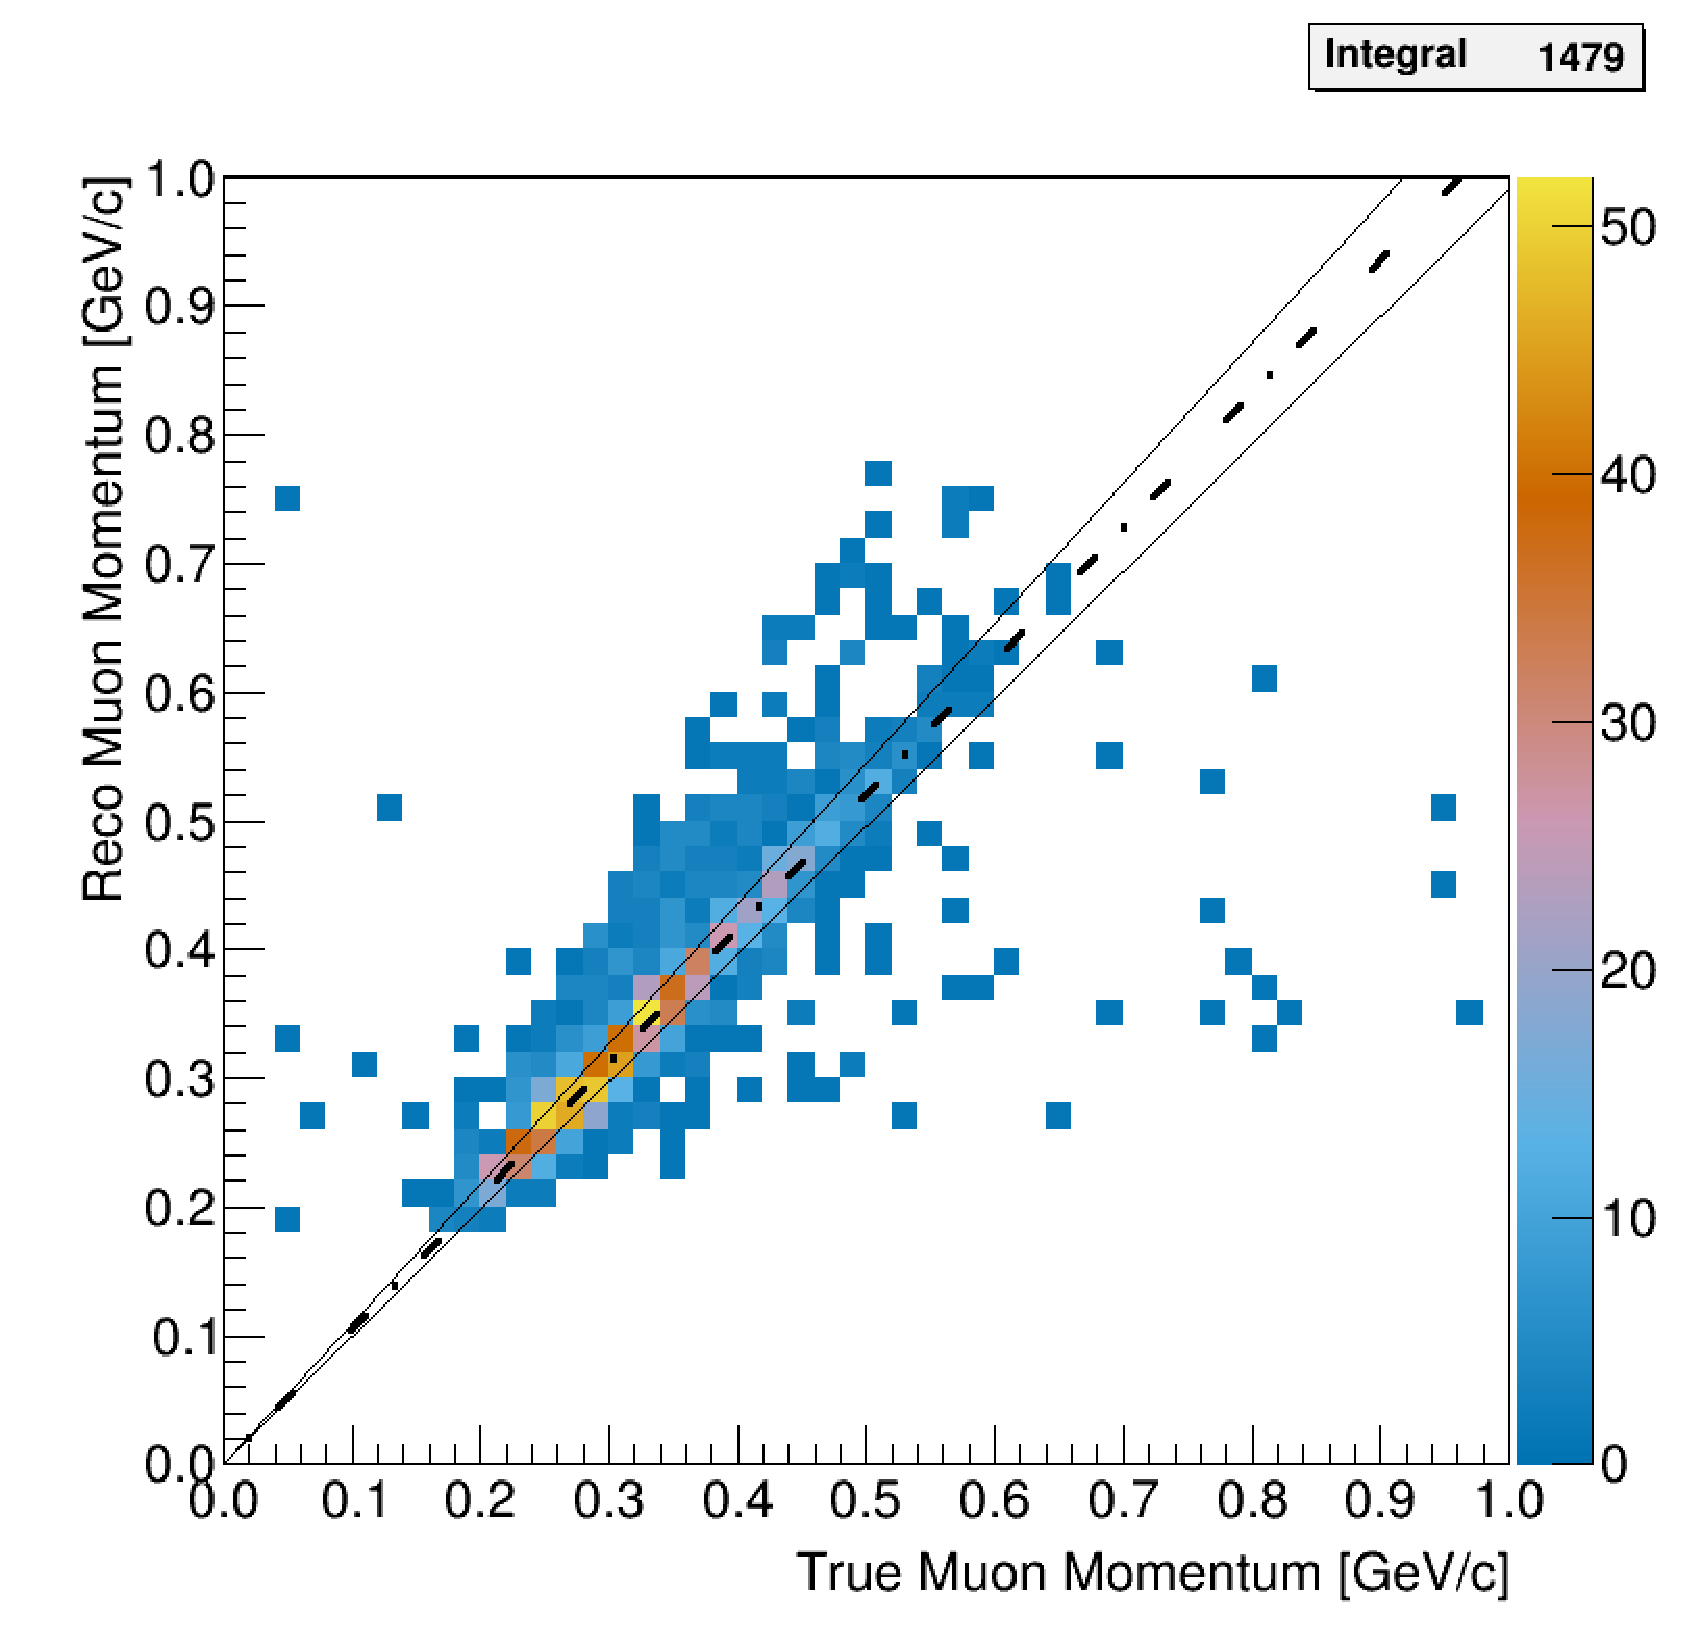
\includegraphics[width=0.48\textwidth]{Appendices/Figures/P0DCC1pi/Contained_SignalMuons_UnCalib_reco_vs_true_p}
            \end{centering}
        }
        \subfloat[Uncalibrated momentum resolution]
        {%
            \begin{centering}
                \includegraphics[width=0.48\textwidth]{Appendices/Figures/P0DCC1pi/Contained_SignalMuons_UnCalib_reco_p_bias}
            \end{centering}
        }
    \end{centering}

    \begin{centering}
        \subfloat[True vs.\ calibrated momentum]
        {%
            \begin{centering}
                \includegraphics[width=0.48\textwidth]{Appendices/Figures/P0DCC1pi/Contained_SignalMuons_Calib_reco_vs_true_p}
            \end{centering}
        }
        \subfloat[Calibrated momentum resolution]
        {%
            \begin{centering}
                \includegraphics[width=0.48\textwidth]{Appendices/Figures/P0DCC1pi/Contained_SignalMuons_Calib_reco_p_bias}
            \end{centering}
        }
        \caption[Momentum Calibration for \podtitle{} Fully Contained Muon Tracks]{The momentum for true muon tracks events before (top) and after (bottom) the calibration. These muon tracks are fully contained in the \podtext{} and are fitted using an algorithm aided by a Kalman filter in the \podtext{} reconstruction. The plots on the left are scatter plots of the true vs.\ reconstructed momentum while the right plots show the resolution of the momentum. After the calibration, the muon tracks have nearly no bias, but at the cost of some additional variance as indicated by the Guassian fits in (b) and (d). The extracted Gaussian fit mean and standard deviation are shown as dashed-dot and solid lines, respectively, in (a) and (c).\label{fig:MuonContainedCalibration}}
    \end{centering}
\end{figure}

\begin{figure}
    \begin{centering}
        \includegraphics[width=0.48\textwidth]{Appendices/Figures/P0DCC1pi/Contained_SignalMuons_NoAnomally_UnCalib_reco_p_biasFit}
        \caption[Resolution Function for \podtitle{} Fully Contained Muon Tracks]{The profile histogram for the
	momentum resolution as function of the reconstructed momentum for \podtext{}
	water-in contained muons. The smooth black curve is a characterization using a logistic function.
    Each bin in the profile has equal statistics to minimize statistical flucuations.\label{fig:MuonContainedResolutionProfile}}
    \end{centering}
\end{figure}
